\documentclass[journal=jctcce,manuscript=article]{achemso}

\usepackage[T1]{fontenc}
\usepackage{graphicx}
\usepackage{amsmath,amssymb}
\usepackage{booktabs}
\usepackage{multirow}
\usepackage{mhchem}
\usepackage[colorlinks=true,citecolor=blue,linkcolor=blue]{hyperref}

\author{Yuan Jiao}
\email{jiaoyuan24@mails.ucas.ac.cn}
\affiliation[UCAS]
{School of Advanced Interdisciplinary Sciences,
 University of Chinese Academy of Sciences, Beijing, China}

\title[GradTDDFT: Differentiable TDDFT Toolkit]
{GradTDDFT: A JAX-Based Differentiable Toolkit for
 Time-Dependent Density Functional Theory with
 Neural Exchange-Correlation Functionals}

\abbreviations{DFT,TDDFT,SCF,XC}
\keywords{differentiable programming, JAX, TDDFT,
neural exchange-correlation functional, excited states}

\begin{document}

\begin{abstract}
We present GradTDDFT, a JAX-based differentiable toolkit
for time-dependent density functional theory (TDDFT) designed
to enable the direct training of neural exchange-correlation
(XC) functionals on excited-state properties. GradTDDFT wraps
a PySCF-compatible electronic structure API in a JAX
differentiable layer, making the full computational graph from
ground-state self-consistent field (SCF) through Casida/TDA
eigensolver to excitation energies and oscillator strengths
amenable to automatic differentiation. A defining feature is
the strict exchange-correlation kernel ($f_{\rm xc}$) computed
as the exact Hessian of the neural XC local energy density via
JAX automatic differentiation, eliminating finite-difference
errors and correctly propagating derivatives through learned
coefficients to density variables. Neural XC functionals can be
trained in a two-stage protocol: ground-state pre-training
against reference energies and densities, followed by
excited-state fine-tuning against excitation energies and
oscillator strengths. Gradient flows through the entire
pipeline---SCF cycle, response matrices, eigensolver, and
observables---are computed automatically via JAX. We validate
the framework through numerical alignment with PySCF reference
calculations and demonstrate neural XC training on the H$_2$
dissociation curve against full configuration interaction
benchmarks. GradTDDFT is released under the Apache 2.0 license
and is freely available on GitHub.
\end{abstract}

\begin{tocentry}
\includegraphics[width=8.5cm]{figures/toc-graphic.pdf}
\end{tocentry}

\section{Introduction}

Density functional theory (DFT) and its linear-response
time-dependent extension (LR-TDDFT) provide efficient routes to
ground-state and excitation energies in molecular electronic
structure.\cite{HohenbergKohn1964,KohnSham1965,RungeGross1984,Casida1995}
Their predictive accuracy is ultimately controlled by the
exchange-correlation (XC) approximation, which must provide not
only an energy but also the derivatives that enter the
self-consistent potential and the response kernel. In Kohn--Sham
DFT, the first functional derivative of the XC energy determines
the XC contribution to the SCF potential; in adiabatic LR-TDDFT,
the second derivative enters the Casida response matrices that
govern excitation energies and oscillator strengths. The XC
functional therefore determines the ground-state SCF reference that
underlies subsequent excited-state response calculations.

Finding a suitable XC functional is therefore
central to reliable ground-state SCF and excited-state response
calculations. Neural network XC functionals provide a flexible route
to learn such functional forms, including nonlocal XC structure,
from accurate reference data.\cite{GLOBE,Schmidt2019NonlocalXCML}
For such excited-state targets, however, fitting ground-state
energies alone is not enough: the functional must also produce
stable self-consistent densities, useful frontier orbital gaps, and
a response kernel consistent with the learned XC energy. This
requirement naturally leads to differentiable training, in which the
functional is optimized through the electronic-structure calculation
that will ultimately use it.\cite{Li2021KohnShamRegularizer} A recent
overview of differentiable DFT emphasizes that this changes the
role of the KS equations: the functional is not only evaluated inside
a self-consistent DFT calculation, but trained through the
differentiable SCF map, with gradients from observables propagated
back to the model parameters while the governing electronic-structure
equations remain in the loop.\cite{vonStrachwitz2026DifferentiableDFT}
For TDDFT, the corresponding differentiable program must extend
beyond the ground-state SCF fixed point to include response-kernel
construction, TDA/Casida eigenvalue problems, excitation energies,
oscillator strengths, and spectrum-level objectives. Differentiable
training is therefore important because it can place losses on the
quantities actually used to judge excited-state predictions, rather
than only on pre-response ground-state energies.

This training view is supported by a broader set of differentiable
algorithms in molecular simulation, semiempirical electronic
structure, quantum chemistry, and materials calculations.\cite{JAXMD,DXTB,Athavale2026DifferentiableSemiempirical,PySCFAD,JRystal,JRystalDirectOptimization,Schmitz2025ADDFPT}
For the present problem, the most relevant progress lies in
differentiable DFT and XC functional construction. DQC and D4FT expose
differentiable DFT workflows for learning or optimizing density
functionals,\cite{DQC,D4FT} GradDFT provides a ground-state framework
for machine-learning enhanced density functionals,\cite{GradDFT} and
jax-xc makes conventional Libxc energy-density forms available as
differentiable functional channels.\cite{JAXXC} In parallel, neural XC
models have explored more flexible functional forms, including
nonlocal and coefficient-basis descriptions beyond a fixed semilocal
ansatz.\cite{Schmidt2019NonlocalXCML,GLOBE,KovacsDLDH2026} Together
these works show how XC functionals can be represented, evaluated, and
trained inside self-consistent DFT calculations. The missing piece for
excited states is an end-to-end differentiable TDDFT formulation in
which the neural XC energy, SCF potential, response kernel, and
excited-state observables belong to the same differentiable
computational graph.

We present GradTDDFT to address this gap by extending GradDFT from
ground-state neural XC functional modeling to differentiable
linear-response TDDFT training. The neural XC model is written as a
coefficient-basis functional with trainable semilocal, HF, and
optional MP2/PT2 channels. Its semilocal basis can be built from
jax-xc energy-density components, so conventional LDA, GGA, and
meta-GGA forms can serve as differentiable functional channels inside
the neural model. GradTDDFT also implements implicit differentiation
for self-consistent ground-state training and excited-state response
training, allowing training objectives to be propagated back to the
XC parameters through the SCF and TDDFT maps. In this way, the
learned XC energy, SCF potential, response kernel, and excited-state
observables are treated within one differentiable training framework.

\section{Theory and Methods}
\label{sec:theory}

% ======================================================================
\subsection{XC Functional Construction}
\label{sec:theory-dft}

For a molecular system with density $\rho$, the Kohn--Sham energy is
written as
\begin{equation}
  E_\theta[\rho]
  =
  T_s[\rho]
  + E_{\rm ne}[\rho]
  + J[\rho]
  + E_{\rm xc}^{\theta}[\rho]
  + E_{\rm nn},
  \label{eq:dft-energy}
\end{equation}
where $T_s$ is the noninteracting kinetic energy, $E_{\rm ne}$ is the
electron--nuclear attraction, $J$ is the Hartree energy, $E_{\rm nn}$
is the nuclear repulsion, and $\theta$ denotes the neural XC
parameters. In an AO basis, the corresponding generalized
eigenvalue problem is
\begin{align}
  \mathbf{F}_\theta[\mathbf{D}]\mathbf{C}
  &=
  \mathbf{S}\mathbf{C}\boldsymbol{\epsilon},
  \label{eq:ks-fock}
  \\
  \mathbf{F}_\theta
  &=
  \mathbf{h}
  + \mathbf{J}[\mathbf{D}]
  + \mathbf{V}_{\rm xc}^{\theta}[\mathbf{D}]
  + \mathbf{V}_{\rm hyb}^{\theta}[\mathbf{D}].
  \nonumber
\end{align}
where $\mathbf{D}$ is the density matrix and
$\mathbf{V}_{\rm hyb}^{\theta}$ collects nonlocal hybrid
contributions.

GradTDDFT uses a coefficient-basis neural hybrid functional. Following
the energy-density mixture idea used in GradDFT,\cite{GradDFT} the XC
energy is written in continuous form as
\begin{align}
  E_{\rm xc}^{\theta}
  &=
  \int e_{\rm xc}^{\theta}(\mathbf{r})\,d\mathbf{r},
  \nonumber
  \\
  e_{\rm xc}^{\theta}(\mathbf{r})
  &=
  \sum_{m=1}^{M}
  c_m^{\theta}(\mathbf{z}(\mathbf{r}))e_m^{\rm sl}(\mathbf{r})
  \nonumber
  \\
  &\quad
  + c_x^{\theta}(\mathbf{z}(\mathbf{r}))h(\mathbf{r})
  + c_2^{\theta}(\mathbf{z}(\mathbf{r}))p(\mathbf{r}) .
  \label{eq:neural-hybrid-functional}
\end{align}
The energy density is expanded into three channel groups: local or
semi-local XC energy densities, a projected local exact-exchange
channel, and an optional projected local MP2/PT2 second-order
correlation channel. Here $\mathbf{z}(\mathbf{r})$ is a local
descriptor vector, $c_m^\theta$, $c_x^\theta$, and $c_2^\theta$ are
learned pointwise mixing fields, $e_m^{\rm sl}(\mathbf{r})$ are
semi-local energy-density channels, $h(\mathbf{r})$ is the local HF
exchange channel density, and $p(\mathbf{r})$ is the local PT2 channel
density. Constant coefficients recover conventional hybrid or
double-hybrid forms, while learned pointwise coefficients define the
neural functional used in GradTDDFT. In numerical calculations,
Eq.~\eqref{eq:neural-hybrid-functional} is evaluated by molecular
quadrature.

A general semi-local channel has the form
\begin{equation}
  e_m^{\rm sl}(\mathbf{r})
  =
  \rho(\mathbf{r})\,
  \varepsilon_m^{\rm sl}
  \!\left(
    \rho_\sigma,
    \nabla\rho_\sigma\!\cdot\!\nabla\rho_{\sigma'},
    \tau_\sigma
  \right),
  \label{eq:semilocal-channel}
\end{equation}
with LDA, GGA, and meta-GGA channels obtained by selecting the
corresponding subset of density variables. For example, a
spin-unpolarized LDA exchange channel and a GGA exchange channel may
be written as
\begin{align}
  e_x^{\rm LDA}(\mathbf{r})
  &=
  -C_x\rho(\mathbf{r})^{4/3},
  \nonumber
  \\
  e_x^{\rm GGA}(\mathbf{r})
  &=
  e_x^{\rm LDA}(\mathbf{r})F_x(s),
  \nonumber
  \\
  s=
  &\,
  \frac{|\nabla\rho(\mathbf{r})|}
       {2(3\pi^2)^{1/3}\rho(\mathbf{r})^{4/3}},
  \label{eq:lda-gga-channel-example}
\end{align}
where $C_x=\frac{3}{4}(3/\pi)^{1/3}$ and $F_x$ is the
functional-specific GGA enhancement factor. Through jax-xc
\cite{JAXXC}, different conventional LDA, GGA, and meta-GGA
energy-density forms can be inserted into the semi-local channel set
without changing the SCF or TDDFT equations.

The HF and MP2/PT2 ingredients enter the coefficient basis through
local channel densities whose integrals recover the conventional
nonlocal energies.  With the spin-density matrix
$\gamma_\sigma(\mathbf{r},\mathbf{r}')$, the exact-exchange channel is
\begin{align}
  E_x^{\rm HF}
  &=
  \int h(\mathbf{r})\,d\mathbf{r}
  =
  -\frac{1}{2}
  \sum_\sigma
  \int
  \frac{
    |\gamma_\sigma(\mathbf{r},\mathbf{r}')|^2
  }{
    |\mathbf{r}-\mathbf{r}'|
  }
  \,d\mathbf{r}\,d\mathbf{r}'
  \nonumber
  \\
  &=
  -\frac{1}{2}
  \sum_{\sigma}
  \sum_{ij\in{\rm occ}_\sigma}
  (ij|ji).
  \label{eq:hf-energy-main}
\end{align}
For the second-order correlation channel, using spin-orbital indices
$i,j$ for occupied orbitals and $a,b$ for virtual orbitals,
\begin{align}
  E_c^{(2)}
  &=
  \int p(\mathbf{r})\,d\mathbf{r}
  =
  -\frac{1}{4}
  \sum_{ijab}
  \frac{
    |\langle ij||ab\rangle|^2
  }{
    D_{ij}^{ab}
  },
  \label{eq:pt2-energy-main}
  \\
  D_{ij}^{ab}
  &=
  \epsilon_a+\epsilon_b-\epsilon_i-\epsilon_j,
  \qquad
  \langle ij||ab\rangle=(ia|jb)-(ib|ja).
  \nonumber
\end{align}
Here $(pq|rs)$ denotes a two-electron integral in chemists'
notation.  The local gauges $h(\mathbf{r})$ and $p(\mathbf{r})$ are
not unique; in GradTDDFT they are projected to the molecular grid as
local HF and PT2 channel features.  Their detailed grid definitions
and response binding are given in the Supporting Information.

% ======================================================================
\subsection{Differentiable SCF and TDDFT}
\label{sec:tddft}

GradTDDFT treats the molecular integrals, basis metadata, and grid
quantities as fixed input data $\mathcal{I}$. The density-dependent
calculation is written as a differentiable SCF fixed point,
\begin{equation}
  \mathbf{D}_\theta^\ast
  =
  \Phi_\theta(\mathbf{D}_\theta^\ast;\mathcal{I}),
  \qquad
  \mathbf{R}_\theta(\mathbf{D})
  =
  \mathbf{D}-\Phi_\theta(\mathbf{D};\mathcal{I}),
  \label{eq:scf-fixed-point-main}
\end{equation}
where $\Phi_\theta$ denotes Fock construction, generalized
diagonalization, occupation assignment, and density reconstruction.
For implicit self-consistent differentiation, the converged density
satisfies $\mathbf{R}_\theta(\mathbf{D}_\theta^\ast)=0$, and its
parameter derivative is obtained from
\begin{equation}
  \frac{d\mathbf{D}_\theta^\ast}{d\theta}
  =
  -
  \left(
    \frac{\partial\mathbf{R}_\theta}{\partial\mathbf{D}}
  \right)^{-1}
  \frac{\partial\mathbf{R}_\theta}{\partial\theta}.
  \label{eq:implicit-main}
\end{equation}
This implicit SCF relation is the ground-state differential used by
the self-consistent training path; alternative fixed-density and
finite-SCF differentiation modes are defined in the Supporting
Information.

After SCF convergence, excitation energies are obtained from
linear-response TDDFT. For occupied orbitals $i,j$ and virtual
orbitals $a,b$, the full Casida equation is
\begin{equation}
  \begin{pmatrix}
    \mathbf{A} & \mathbf{B} \\
    \mathbf{B} & \mathbf{A}
  \end{pmatrix}
  \begin{pmatrix}
    \mathbf{X}_I \\
    \mathbf{Y}_I
  \end{pmatrix}
  =
  \Omega_I
  \begin{pmatrix}
    \mathbf{1} & \mathbf{0} \\
    \mathbf{0} & -\mathbf{1}
  \end{pmatrix}
  \begin{pmatrix}
    \mathbf{X}_I \\
    \mathbf{Y}_I
  \end{pmatrix},
  \label{eq:casida-main}
\end{equation}
where $\Omega_I$ is the excitation energy. The response matrices have
the schematic form
\begin{equation}
  \begin{aligned}
  A_{ia,jb}
  &=
  (\epsilon_a-\epsilon_i)\delta_{ij}\delta_{ab}
  + K_{ia,jb},
  \\
  B_{ia,jb}
  &=
  K_{ia,bj},
  \end{aligned}
  \label{eq:ab-main}
\end{equation}
where $K$ contains Coulomb, XC-kernel, and hybrid-response
contributions. The Tamm--Dancoff approximation sets
$\mathbf{B}=0$ and gives
\begin{equation}
  \mathbf{A}\mathbf{X}_I=\Omega_I\mathbf{X}_I .
  \label{eq:tda-main}
\end{equation}

The differentiable link between the SCF energy and the TDDFT response
is the XC kernel. For the local and semi-local part,
\begin{equation}
  f_{\rm xc}^{\theta}(\mathbf{r},\mathbf{r}')
  =
  \frac{\delta^2 E_{\rm xc}^{\theta}}
       {\delta\rho(\mathbf{r})\delta\rho(\mathbf{r}')}.
  \label{eq:fxc-main}
\end{equation}
Thus the SCF potential and the local response kernel are derivatives
of the same energy-density model. In GradTDDFT these derivatives are
evaluated by automatic differentiation of the pointwise energy
density, so derivatives of the learned mixing fields are included in
both the potential and the TDDFT kernel. The nonlocal HF response,
the PT2 excited-state correction, and optional RI response
contractions are specified in the Supporting Information.

For differentiable excited-state training, the response problem is
evaluated at the implicit SCF solution $\mathbf{D}_\theta^\ast$. The
TDDFT root derivative therefore contains both the explicit derivative
of the response operator and the implicit derivative of the converged
density in Eq.~\eqref{eq:implicit-main}. In the Davidson response
solver, GradTDDFT follows the implicit eigensolver differentiation
strategy of Xie, Liu, and Wang,\cite{Xie2020DominantEigensolverAD}
using the converged Ritz amplitudes to reconstruct the root-energy
differential rather than differentiating through the full iteration
history. For the TDA operator, this takes the Rayleigh-quotient form
\begin{equation}
  d\Omega_I
  =
  \frac{
    \mathbf{X}_I^{T}
    (d\mathbf{A})
    \mathbf{X}_I
  }{
    \mathbf{X}_I^{T}\mathbf{X}_I
  },
  \label{eq:tda-root-differential-main}
\end{equation}
with $d\mathbf{A}$ including both direct neural-kernel derivatives and
the SCF response from Eq.~\eqref{eq:implicit-main}. The corresponding
full Casida expression is given in the Supporting Information.

\section{Implementation}
\label{sec:implementation}

The implementation follows the same design principle that underlies
GradDFT\cite{GradDFT}: fixed electronic-structure inputs are separated
from the differentiable program that evaluates energies,
self-consistent fields, response matrices, and losses.
For GradTDDFT the distinction is extended to excited-state response.
Molecular preprocessing constructs the fixed numerical representation
of a calculation, while the differentiable core operates on density
matrices, orbital rotations, local density variables, and neural
functional parameters.

% ======================================================================
\subsection{Molecular State and Fixed Data}

A GradTDDFT calculation begins from the same physical inputs as a
conventional KS or TDDFT calculation: nuclear charges and coordinates,
charge, spin, basis set, exchange-correlation functional, quadrature
grid, and convergence settings. PySCF is used to construct the
molecule, basis metadata, quadrature grid, AO values on grid points,
one-electron integrals, and electron-repulsion data. These quantities
are then treated as fixed arrays during the differentiable SCF and
response calculation. This boundary keeps the integral and grid
generation path aligned with PySCF reference calculations while
placing the density-dependent part of the method inside JAX.

The fixed molecular state contains the overlap matrix $S$, core
Hamiltonian $h$, grid weights, AO values and derivatives, nuclear
repulsion energy, and the selected representation of the two-electron
integrals. GradTDDFT supports dense electron-repulsion tensors,
density-fitted contractions, and direct J/K construction. The choice
of J/K backend changes how Coulomb and exchange contractions are
formed, but not the mathematical objects passed to the SCF or TDDFT
layers.

% ======================================================================
\subsection{Differentiable SCF and TDDFT Execution}

After molecular preprocessing, the SCF layer is evaluated entirely as
a differentiable fixed-point computation. For a density matrix $P$,
the implementation assembles
\begin{equation}
  F[P;\theta]
  =
  h + J[P] + F_{\rm xc}[P;\theta] + F_{\rm nl}[P;\theta],
\end{equation}
where $J[P]$ is the Coulomb contribution, $F_{\rm xc}$ is the
semilocal or neural XC potential, and $F_{\rm nl}$ denotes optional
nonlocal HF and MP2/PT2-channel contributions. The SCF map diagonalizes
the generalized eigenvalue problem, updates occupations and density,
and repeats this operation until the selected convergence criteria are
satisfied. The converged state stores orbitals, orbital energies,
occupations, density matrices, total energies, and diagnostic
residuals needed by both response calculations and training losses.

The differentiable program can be evaluated either through an
explicit finite SCF trace or through an implicit fixed-point
gradient. Both modes use the same molecular state and Fock-building
path. This is important for comparing training objectives: changes in
the gradient treatment should not change the forward SCF solution
used to build the TDDFT response problem.

The TDDFT layer is differentiated in the same operator-first spirit.
For a converged SCF state, the implementation builds matrix actions
for the TDA or full Casida response problem from orbital-energy
differences, Coulomb and exchange contractions, semilocal XC response
actions, and nonlocal neural-channel response terms. During training,
the Davidson solver is used only as the forward numerical procedure
for obtaining the requested low-lying roots. Following the implicit
differentiation formulation for iterative eigensolvers by Lei Wang and
co-workers,\cite{Xie2020DominantEigensolverAD} GradTDDFT uses a
differentiable Davidson mode in which the reverse-mode derivative
is not taken through the Davidson iteration history, but through the
stationarity of the converged Ritz pairs. In practice, the
matrix-vector products used inside the Davidson iterations are
detached from the reverse pass. After convergence, the Ritz
amplitudes are also held fixed and the excitation energy is
reconstructed as a Rayleigh quotient of the current response
operator. Gradients of excitation-energy losses therefore flow
through the response matrix-action builder, the SCF fixed point, and
the neural functional parameters, while avoiding a large
differentiation tape for the iterative eigensolver. Oscillator
strengths and broadened spectra are evaluated from the same forward
roots; their present training path does not include an additional
eigenvector-response derivative beyond this fixed-amplitude
reconstruction. Detailed formulas for the TDA and Casida root-energy
derivatives are given in the Supporting Information.

% ======================================================================
\subsection{Functional Evaluation and Response Core}

The functional interface is organized around a local energy-density
map. For traditional semilocal functionals, the map evaluates a
specified LDA, GGA, or meta-GGA energy density on the grid. For
neural functionals, local density descriptors are combined with
learned coefficient fields that mix semilocal, HF, and optional MP2/PT2
channels. In both cases the scalar XC energy is obtained by numerical
quadrature, and the SCF potential follows from differentiating the
same energy expression with respect to the density variables.

The conventional semilocal energy-density components are evaluated
through the JAX-XC functional library,\cite{JAXXC} with hybrid exact
exchange handled by the nonlocal HF channel. JAX-XC provides a broader
catalogue of Libxc-translated LDA, GGA, meta-GGA, and hybrid functional
routines than the subset used below. For the GradTDDFT implementation
and the calculations in this manuscript, the default validated
functional inputs include:
\begin{itemize}
  \item LDA and local-correlation components: LDA exchange,
    Perdew--Wang correlation, Vosko--Wilk--Nusair correlation, and
    the VWN-RPA variant.
  \item GGA components: Becke 88 exchange, PBE exchange, the
    range-separated PBE exchange component, LYP correlation, and PBE
    correlation.
  \item Composite local and semilocal specifications: LDA, SVWN,
    SVWN-RPA, PBE, and the local semilocal part of LC-WPBE.
  \item Global and screened hybrid specifications: PBE0/PBEH, B3LYP,
    BHandHLYP, HSE03, and HSE06. Their semilocal terms are routed
    through JAX-XC, while the HF fraction is assembled by the exact
    exchange contraction path.
\end{itemize}
Additional installed JAX-XC names, including further GGA, meta-GGA,
and hybrid components, can be routed as optional channels after
validation for the selected SCF and TDDFT response path. They are not
part of the default validated set used for the calculations described
here.

The TDDFT response layer reuses the converged SCF state and constructs
the TDA or full Casida matrices from orbital-energy differences,
Coulomb and exchange response contractions, and the XC kernel. For
semilocal response, the local kernel is the Hessian of the same
energy-density map used for the SCF potential. This gives a single
source for $E_{\rm xc}$, $v_{\rm xc}$, and $f_{\rm xc}$ rather than
three separately implemented formulas. The corresponding data flow for
traditional functionals is summarized in
Figure~\ref{fig:traditional-response-core}.

\begin{figure}
  \centering
  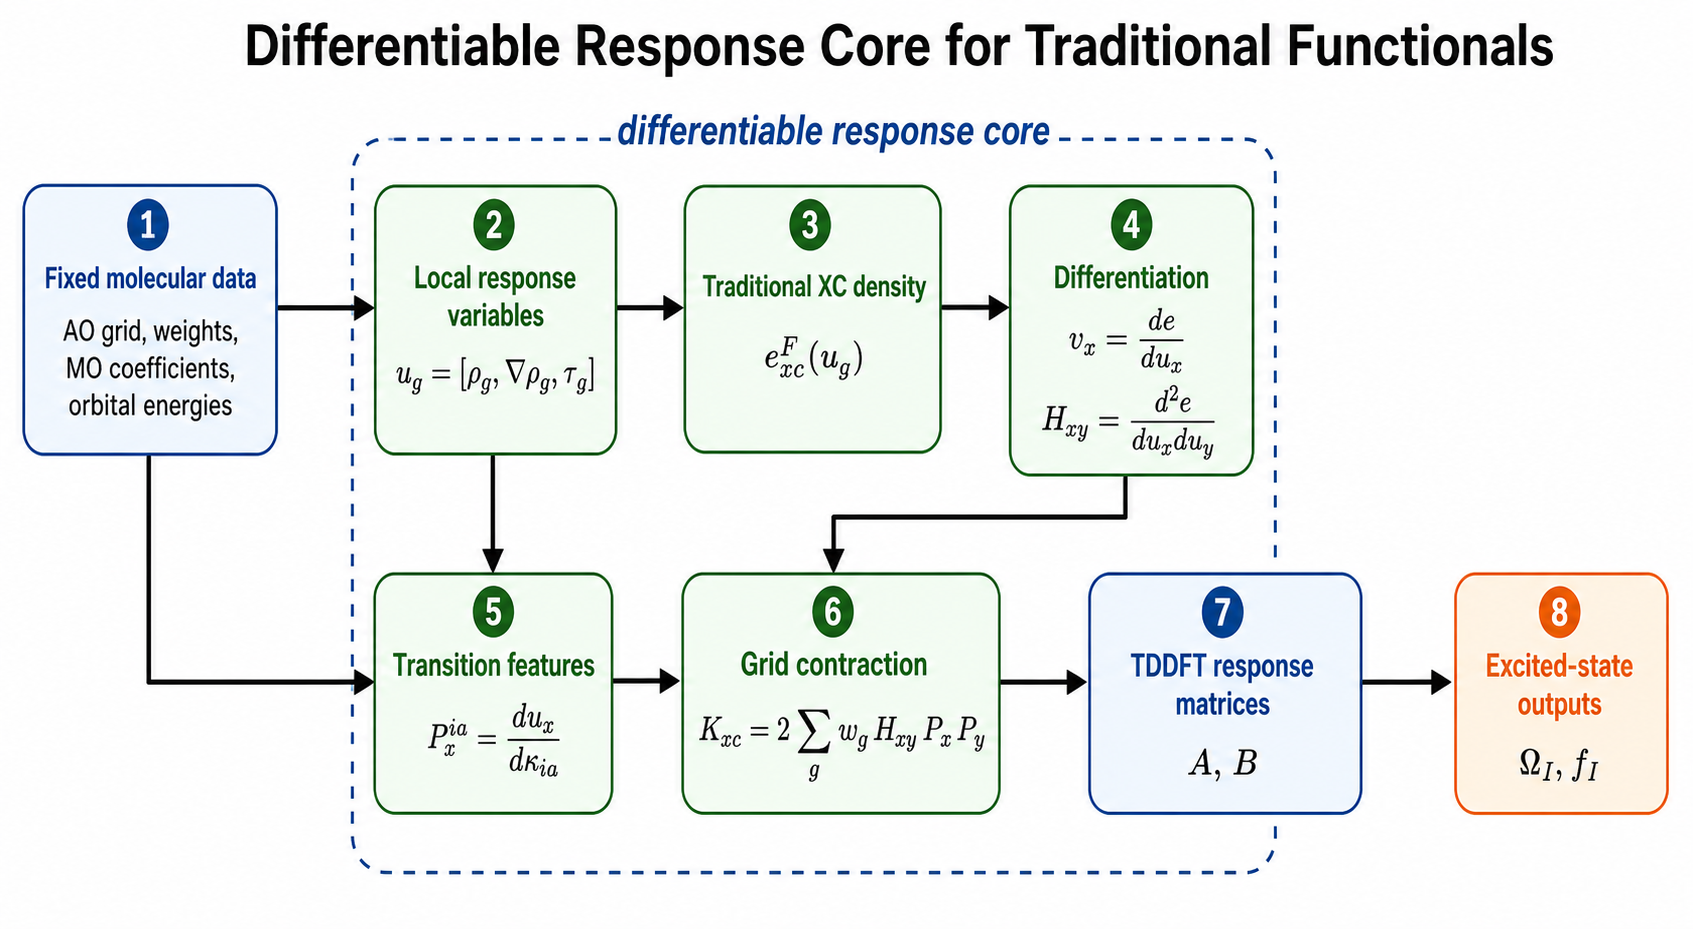
\includegraphics[width=\linewidth]{figures/figure3-traditional-response-core-gpt-image2.png}
  \caption{Differentiable response-core construction for traditional
    semilocal functionals. Fixed molecular data define local density
    variables and transition response features, while differentiation
    of the XC energy density supplies the potential and local Hessian
    used to assemble TDDFT response matrices.}
  \label{fig:traditional-response-core}
\end{figure}

For the neural HF channel, the response binding converts the learned
local exchange field into a density-weighted scalar exchange fraction
and inserts it into the same nonlocal exact-exchange contractions used
by hybrid TDDFT. For the neural MP2/PT2 channel, the response solver
first obtains the TDA or Casida singles roots and then applies a
state-specific CIS(D)-type second-order correction scaled by the
learned PT2 coefficient. This is the calculation path used for the
excited-state tests described in Section~\ref{sec:results}.

% ======================================================================
\subsection{Training and Observable Evaluation}

The final computational graph maps neural parameters to scalar losses.
Starting from the fixed molecular state, GradTDDFT performs SCF,
constructs the response matrices, solves the TDA or full TDDFT
eigenvalue problem, and evaluates observables such as excitation
energies, oscillator strengths, transition dipoles, state-ordering
metrics. Figure~\ref{fig:computation-flow}
summarizes this end-to-end path.

\begin{figure}
  \centering
  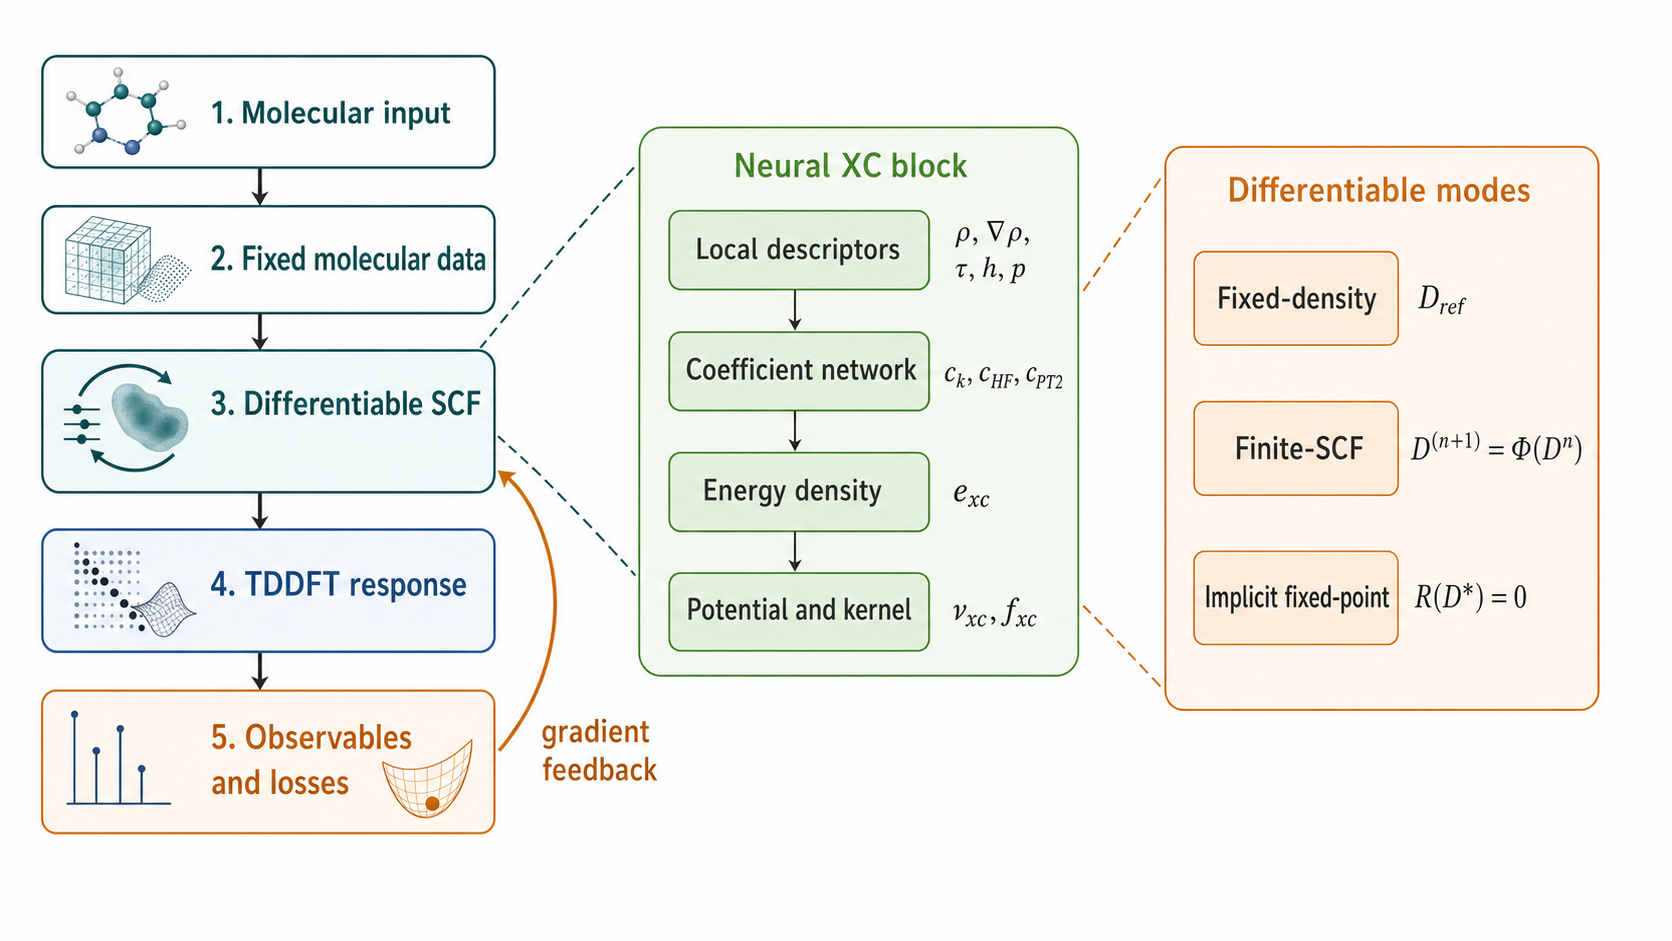
\includegraphics[width=\linewidth]{figures/figure2-computation-flow-sphnet-style-gpt-image2.png}
  \caption{End-to-end computation flow for differentiable
    ground-state and excited-state training.
    Fixed molecular data are passed through SCF and TDDFT response
    construction to produce observables and scalar losses whose
    gradients propagate back to the neural functional parameters.}
  \label{fig:computation-flow}
\end{figure}

Loss terms can target ground-state energies, excitation energies,
oscillator strengths, or state-ordering diagnostics. The current
training protocol optimizes ground-state and excited-state objectives
in separate runs.
Each calculation records the SCF convergence
status, response solver, excited-state treatment, backend, seed, and reference
labels. These records separate numerical failures from functional
errors.

% ======================================================================
\subsection{Verification}

Verification uses matched PySCF calculations and gradient audits.
Runs with traditional functionals compare SCF energies, orbital
energies, TDA and full TDDFT excitation energies, oscillator
strengths, transition dipoles, and response-matrix components against
PySCF references. The matched settings include geometry, basis, grid,
functional, and spin treatment. These tests establish that the
differentiable path reproduces the reference TDDFT calculation before
neural parameters are introduced.

Differentiability audits evaluate representative scalar losses through
the full SCF, response, and observable graph. The audits check finite
values, finite gradients, and nonzero parameter sensitivity. They are
run for explicit finite-SCF differentiation and implicit fixed-point
gradients, together with implicit TDDFT root differentiation, ensuring
that the implementation can support the training paradigms described
in Section~\ref{sec:theory}.

\section{Computational Evaluation}
\label{sec:results}

The computational evaluation begins with a numerical validation
against PySCF and then turns to model-capability tests. The validation
module checks that GradTDDFT reproduces conventional TDA and full
TDDFT excitation energies, oscillator strengths, and response
matrices before neural parameters are introduced. The capability
tests then ask whether differentiable neural exchange-correlation
functionals can learn ground-state surfaces, excited-state response,
and molecular ground-state and vertical-excitation targets
within a shared SCF--TDDFT implementation. These model tests are
divided into two blocks: bond-dissociation curves covering
ground-state surfaces and first excited-state response, and
separate ground-state and excited-state training on a 50-molecule QM9
subset.

Across all experiments, the recorded computational state includes the
geometry source, charge and spin multiplicity, basis set, quadrature
grid, SCF convergence criteria, TDDFT solver, excited-state treatment,
backend/device, training seed, and reference method. These records are
part of the benchmark definition because small changes in grids,
spin treatment, or SCF convergence can otherwise obscure whether an
observed error comes from the learned functional or from the numerical
setup.

% ======================================================================
\subsection{Numerical Validation against PySCF}
\label{sec:eval-pyscf}

The first evaluation module isolates the TDDFT response construction
before any neural functional parameters are trained. In the
conventional-functional limit, GradTDDFT evaluates the
exchange-correlation energy density as a differentiable function of
the density descriptors and obtains both the potential and the local
response tensor by automatic differentiation,
\begin{equation}
  E_{\rm xc}
  \longrightarrow
  v_{\rm xc}
  =
  \frac{\delta E_{\rm xc}}{\delta \rho}
  \longrightarrow
  f_{\rm xc}
  =
  \frac{\delta v_{\rm xc}}{\delta \rho}.
\end{equation}
The resulting tensor is contracted with quadrature weights and AO
basis values, transformed to the occupied--virtual orbital basis, and
inserted into the TDA or Casida response matrices. Matched PySCF
calculations provide independent references for the same geometry,
functional, basis, grid, SCF solution, and response equations.

The validation matrix contains H$_2$O, CO, N$_2$, C$_2$H$_4$,
formaldehyde, benzene, and OH with PBE, B3LYP, and PBE0 in def2-SVP
and aug-cc-pVDZ basis sets. Restricted KS references are used for the
closed-shell molecules, while unrestricted KS references are used for
OH. For each matched setup, TDA and full TDDFT are evaluated for the
first five singlet and triplet states where the reference calculation
is defined.

For the PBE/def2-SVP subset reported here, all 26 calculations
completed successfully, giving 130 per-state records. The direct
GradTDDFT--PySCF comparison contains 12 restricted-singlet tasks,
corresponding to 60 excitation states across TDA and full TDDFT. The
excitation-energy mean absolute differences relative to PySCF range
from \(5.86\times 10^{-14}\) to \(2.87\times 10^{-10}\) eV, with
maximum absolute state errors below \(5.47\times 10^{-10}\) eV.
Oscillator-strength mean absolute differences range from
\(1.86\times 10^{-22}\) to \(1.29\times 10^{-7}\). For response
matrices small enough to store explicitly in this audit, the RMS
differences in the assembled \(A\) and \(B\) matrices are
\(5.65\times 10^{-15}\) to \(8.26\times 10^{-15}\).

\begin{table}[t]
\centering
\caption{B3LYP/def2-SVP S$_1$ excitation energies and oscillator
strengths from matched PySCF and GradTDDFT calculations. Each entry
reports \(\Omega_1\) in eV followed by \(f_1\).}
\label{tab:b3lyp-s1-excitation-oscillator}
\begin{tabular}{llcc}
\toprule
Molecule & Solver & PySCF & GradTDDFT \\
\midrule
H$_2$O & TDA & 7.6 / \(1.8\times 10^{-2}\) & 7.6 / \(1.8\times 10^{-2}\) \\
H$_2$O & TDDFT & 7.6 / \(1.8\times 10^{-2}\) & 7.6 / \(1.8\times 10^{-2}\) \\
CO & TDA & 8.7 / \(1.1\times 10^{-1}\) & 8.7 / \(1.1\times 10^{-1}\) \\
CO & TDDFT & 8.5 / \(8.2\times 10^{-2}\) & 8.5 / \(8.2\times 10^{-2}\) \\
N$_2$ & TDA & 9.5 / \(4.5\times 10^{-31}\) & 9.5 / \(3.4\times 10^{-31}\) \\
N$_2$ & TDDFT & 9.4 / \(4.7\times 10^{-18}\) & 9.4 / \(7.2\times 10^{-25}\) \\
C$_2$H$_4$ & TDA & 8.3 / \(5.4\times 10^{-29}\) & 8.3 / \(6.0\times 10^{-29}\) \\
C$_2$H$_4$ & TDDFT & 8.1 / \(3.7\times 10^{-1}\) & 8.1 / \(3.7\times 10^{-1}\) \\
CH$_2$O & TDA & 4.0 / \(1.9\times 10^{-29}\) & 4.0 / \(1.8\times 10^{-29}\) \\
CH$_2$O & TDDFT & 4.0 / \(2.2\times 10^{-25}\) & 4.0 / \(5.4\times 10^{-29}\) \\
C$_6$H$_6$ & TDA & 5.5 / \(3.7\times 10^{-9}\) & 5.5 / \(3.7\times 10^{-9}\) \\
C$_6$H$_6$ & TDDFT & 5.5 / \(4.9\times 10^{-9}\) & 5.5 / \(4.9\times 10^{-9}\) \\
\bottomrule
\end{tabular}
\end{table}

This validation establishes the numerical equivalence of the
differentiable TDDFT path and matched PySCF calculations for
traditional functionals. The following sections therefore evaluate
model behavior rather than basic response-matrix assembly.

% ======================================================================
\subsection{\texorpdfstring{Ground- and Excited-State Dissociation Curves}{Ground- and Excited-State Dissociation Curves}}
\label{sec:eval-dissociation}
\label{sec:eval-ground-dissociation}
\label{sec:eval-excited-dissociation}

The first model-capability benchmark evaluates one-dimensional bond
dissociation curves for H$_2$, H$_2^+$, and N$_2$, with first
excited-state scans for H$_2$ and N$_2$. The H$_2$/H$_2^+$
pair follows the Kohn--Sham regularizer benchmark of Li
\emph{et al.}: H$_2$ is a compact bond-breaking and
strong-correlation test, whereas H$_2^+$ isolates one-electron
self-interaction and open-shell SCF stability.\cite{Li2021KohnShamRegularizer}
N$_2$ extends this setting to a stretched multiple bond; recent
high-level spectroscopic calculations treat molecular nitrogen as a
dense multi-state problem, reporting potential-energy curves and
transition dipole moments for the 51 lowest electronic states over
1.35--10 bohr and multiple N + N dissociation
limits.\cite{Hammami2026N2PEC} The three systems therefore separate
self-interaction, two-electron bond breaking, and stretched
triple-bond near-degeneracy within a small set of scans.
The ground-state curves are labeled by the corresponding
diatomic spectroscopic terms, \(X\,{}^1\Sigma_g^+\) for H$_2$
and N$_2$ and \(X\,{}^2\Sigma_g^+\) for H$_2^+\). The excited-state
curves are labeled as H$_2$ \(B\,{}^1\Sigma_u^+\) and N$_2$
\(A\,{}^1\Pi_g\); the latter follows the large-CAS state assignment
used in the N$_2$ reference data.\cite{Hammami2026N2PEC}

The results are organized around the physically meaningful channel for
each system. For the one-electron H$_2^+$ ion, the MP2/PT2 doubles
space is empty, so a PT2 correction is identically zero and does not
provide a useful functional test. H$_2^+$ is therefore used to compare
implicit-SCF training with fixed-density training. For H$_2$ and N$_2$,
the implicit-SCF protocol is used throughout, and the PT2/no-PT2
comparison tests how strongly the second-order channel improves the
learned functional along bond dissociation. The H$_2$ and N$_2$ first
excited-state dissociation curves apply the same PT2-channel test to
the TDDFT response calculation. The curve-plus-error layout, training
markers, and chemical accuracy band are used as direct diagnostics,
with convergence success, cycle count, and failure rate recorded at
every geometry.

\begin{figure}[!htbp]
\centering
\begin{minipage}{0.49\linewidth}
  \centering
  \textbf{(a) Implicit SCF}\\[-0.3em]
  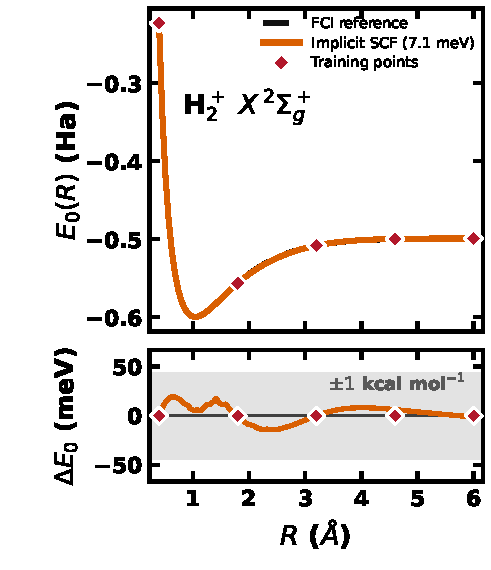
\includegraphics[width=\linewidth]{figures/h2plus_ground_hfx_implicit_scf_dissociation_paper_style.pdf}
\end{minipage}
\hfill
\begin{minipage}{0.49\linewidth}
  \centering
  \textbf{(b) Fixed density}\\[-0.3em]
  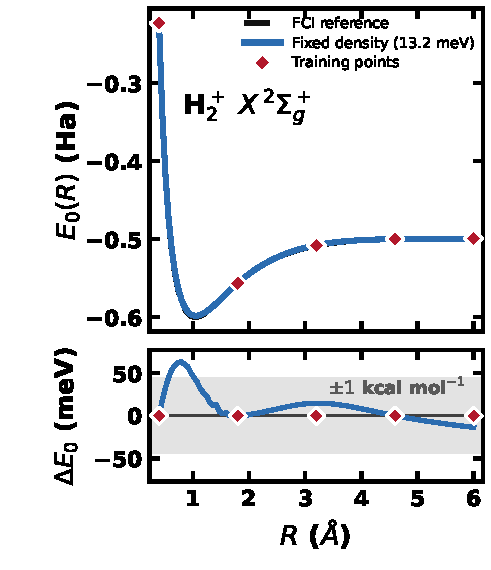
\includegraphics[width=\linewidth]{figures/h2plus_ground_hfx_fixed_density_dissociation_paper_style.pdf}
\end{minipage}
\caption{H$_2^+$ \(X\,{}^2\Sigma_g^+\) ground-state dissociation
curves for the HFX-channel neural functional under implicit-SCF and
fixed-density training. In
each panel, the upper subpanel compares the learned curve with the
one-electron FCI reference values, while the lower subpanel shows the
signed error
\(\Delta E_0=E_{0,\rm model}-E_{0,\rm ref}\). Red diamonds denote the
five training geometries, and the gray band marks
\(\pm 1\) kcal mol\(^{-1}\). The implicit-SCF model gives a dense-curve
mean absolute error of 7.1 meV and a maximum absolute error of
19.2 meV. Fixed-density training gives corresponding errors of
13.2 meV and 63.2 meV.}
\label{fig:h2plus-ground-hfx-dissociation}
\end{figure}

\begin{figure}[!htbp]
\centering
\begin{minipage}{0.485\linewidth}
  \centering
  \textbf{(a) H$_2$, HFX+PT2}\\[-0.3em]
  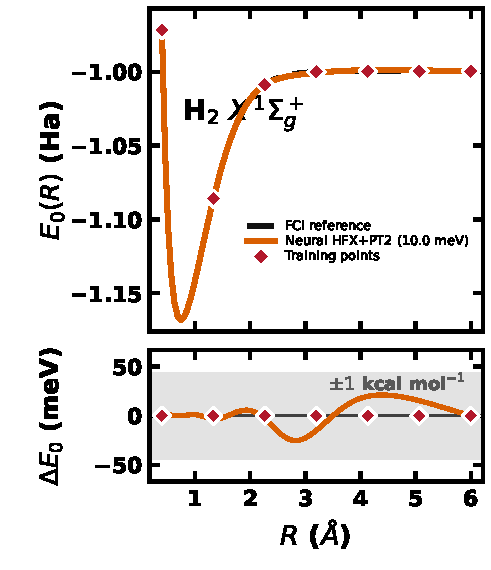
\includegraphics[width=0.88\linewidth]{figures/h2_ground_hfx_pt2_dissociation_paper_style.pdf}
\end{minipage}
\hfill
\begin{minipage}{0.485\linewidth}
  \centering
  \textbf{(b) H$_2$, HFX/no-PT2}\\[-0.3em]
  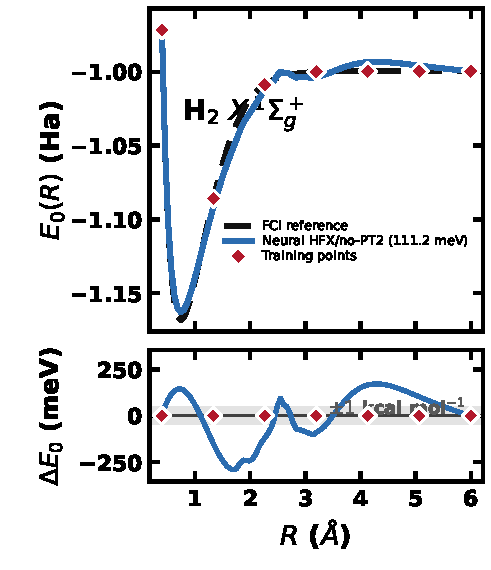
\includegraphics[width=0.88\linewidth]{figures/h2_ground_hfx_nopt2_dissociation_paper_style.pdf}
\end{minipage}\\[-0.2em]
\begin{minipage}{0.485\linewidth}
  \centering
  \textbf{(c) N$_2$, HFX+PT2}\\[-0.3em]
  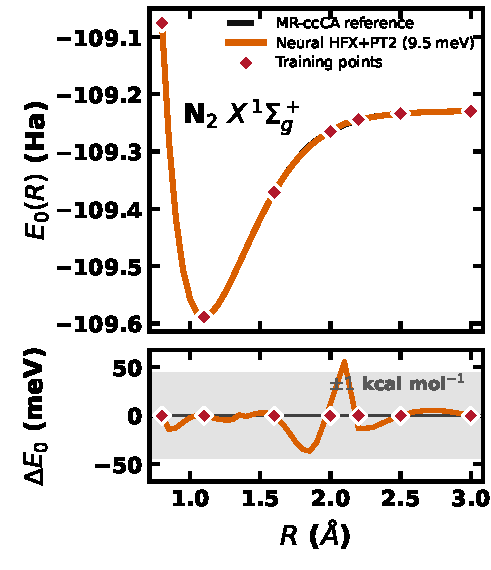
\includegraphics[width=0.88\linewidth]{figures/n2_ground_hfx_pt2_dissociation_paper_style.pdf}
\end{minipage}
\hfill
\begin{minipage}{0.485\linewidth}
  \centering
  \textbf{(d) N$_2$, HFX/no-PT2}\\[-0.3em]
  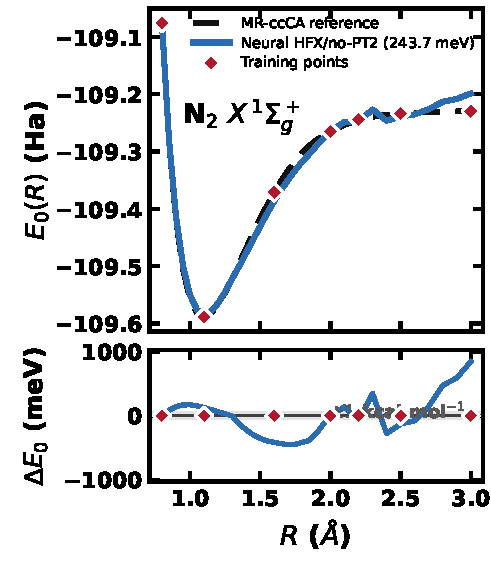
\includegraphics[width=0.88\linewidth]{figures/n2_ground_hfx_nopt2_dissociation_paper_style.pdf}
\end{minipage}
\caption{H$_2$ and N$_2$ \(X\,{}^1\Sigma_g^+\) ground-state
dissociation curves for neural functionals trained with and without
the PT2 channel. In each panel,
the upper subpanel compares the learned curve with the reference
values, while the lower subpanel shows the signed error
\(\Delta E_0=E_{0,\rm model}-E_{0,\rm ref}\). Red diamonds denote the
seven training geometries, and the gray band marks
\(\pm 1\) kcal mol\(^{-1}\). For H$_2$, the HFX+PT2 model gives a
dense-curve mean absolute error of 10.0 meV and a maximum absolute
error of 25.4 meV, while removing the PT2 channel increases the
corresponding errors to 111.2 meV and 292.1 meV. For N$_2$, the
HFX+PT2 model gives corresponding errors of 9.5 meV and 55.7 meV,
whereas the HFX/no-PT2 model gives 243.7 meV and 844.0 meV.}
\label{fig:h2-n2-ground-hfx-pt2-nopt2-dissociation}
\label{fig:h2-ground-hfx-pt2-nopt2-dissociation}
\label{fig:n2-ground-hfx-pt2-nopt2-dissociation}
\end{figure}

\begin{figure}[!htbp]
\centering

\includegraphics[width=0.86\linewidth]{figures/h2_s1_tda_e1_total_pt2_nopt2_dissociation_paper_style.pdf}
\caption{H$_2$ \(B\,{}^1\Sigma_u^+\) excited-state dissociation curve
for neural TDA calculations with and without the PT2 channel. The
plotted quantity is the total excited-state energy
\(E_1(R)=E_0(R)+\Omega_1(R)\). In each panel, the upper subpanel
compares the learned curve with the FCI reference values, while the
lower subpanel shows the signed error
\(\Delta E_1=E_{1,\rm model}-E_{1,\rm ref}\). Red diamonds denote the
training geometries, and the gray band marks
\(\pm 1\) kcal mol\(^{-1}\). The PT2-channel model gives a dense-curve
mean absolute error of 35.9 meV and a maximum absolute error of
208.0 meV, whereas the updated no-PT2 model gives corresponding
errors of 70.1 meV and 199.3 meV.}
\label{fig:h2-s1-tda-e1-total-pt2-nopt2-dissociation}
\end{figure}

\begin{figure}[!htbp]
\centering

\includegraphics[width=0.86\linewidth]{figures/n2_s1_tda_e1_total_pt2_nopt2_dissociation_paper_style.pdf}
\caption{N$_2$ \(A\,{}^1\Pi_g\) excited-state dissociation curves for
neural TDA calculations with and without the PT2 channel. The plotted
quantity is the total excited-state energy
\(E_1(R)=E_0(R)+\Omega_1(R)\), using the Hammami
\emph{et al.} large-CAS curve as the reference.\cite{Hammami2026N2PEC}
In each panel, the upper subpanel compares the learned
curve with the reference values, while the lower subpanel shows the
signed error
\(\Delta E_1=E_{1,\rm model}-E_{1,\rm ref}\). Red diamonds denote the
training geometries, and the gray band marks
\(\pm 1\) kcal mol\(^{-1}\). The PT2-channel model gives a dense-curve
mean absolute error of 0.161 eV and a maximum absolute error of
0.477 eV, while removing the PT2 channel increases the corresponding
errors to 0.871 eV and 2.905 eV.}
\label{fig:n2-s1-tda-e1-total-pt2-nopt2-dissociation}
\end{figure}

\subsection{Semi-local Channel Composition Tests}
\label{sec:semilocal-channel-composition}

The dissociation benchmarks above vary the implicit-SCF treatment and
the second-order PT2 channel. A complementary training test asks a
narrower question: under a fixed \texttt{noPT2}+HFX implicit-SCF
protocol, how strongly does the semi-local channel basis affect the
N$_2$ ground-state and first-excited-state dissociation curves? In
this comparison, the MP2/PT2 channel is disabled, the local
exact-exchange descriptor \(h_g\) remains active through
\(c_x^\theta(\mathbf{z}_g)h_g\), and only the set of semi-local energy
densities \(\{e_m^{\rm sl}\}\) in Eq.~\ref{eq:semilocal-channel} is
changed. The neural architecture, optimizer, training geometries,
quadrature grid, and implicit differentiation of the SCF--TDDFT
workflow are kept fixed.

We refer to these models as semi-local channel-composition variants.
The functional labels identify the JAX-XC energy-density components
used to build the coefficient basis; they do not introduce fixed
parent-functional mixing fractions. Because this benchmark uses the
\texttt{noPT2} setting, no \(c_2^\theta(\mathbf{z}_g)p_g\) contribution
is included. The comparison therefore isolates how LDA, GGA, and
meta-GGA semi-local priors interact with the learned local HFX channel
in the coefficient-basis form of
Eq.~\ref{eq:neural-hybrid-functional}.

\begin{table}[t]
\centering
\caption{Semi-local channel-composition benchmark for N$_2$
dissociation. The MP2/PT2 channel is disabled, the local HFX channel
is enabled, and all variants use the implicit-SCF training path. Only
the semi-local basis \(\{e_m^{\rm sl}\}\) is changed.}
\label{tab:semilocal-channel-composition}
\begin{tabular}{p{0.20\linewidth}p{0.36\linewidth}p{0.34\linewidth}}
\toprule
Variant & Semi-local channel basis & Dissociation diagnostic \\
\midrule
\texttt{lda\_vwn\_rpa} &
\texttt{lda\_x} + \texttt{lda\_c\_vwn\_rpa} &
Baseline for \(E_0(R)\) and \(E_1(R)\) \\
\texttt{gga\_pbe} &
\texttt{gga\_x\_pbe} + \texttt{gga\_c\_pbe} &
GGA exchange/correlation prior \\
\texttt{mgga\_r2scan} &
\texttt{mgga\_x\_r2scan} + \texttt{mgga\_c\_r2scan} &
Meta-GGA \(\tau\)-dependent prior \\
\bottomrule
\end{tabular}
\end{table}

Each variant is trained and evaluated with the same N$_2$ geometries,
reference labels, basis/grid settings, and response solver. The
ground-state comparison uses \(E_0(R)\); the excited-state comparison
uses the first excitation energy \(\Omega_1(R)\) and the total
first-excited-state curve \(E_1(R)=E_0(R)+\Omega_1(R)\). Since HFX is
enabled and PT2 is disabled in all rows of
Table~\ref{tab:semilocal-channel-composition}, differences across the
three variants are attributed to the semi-local channel basis rather
than to changes in the nonlocal response ingredients.

Within the same dissociation benchmark, training on near-equilibrium
geometries is compared with training on the full curve. The
near-equilibrium regime tests extrapolation into stretched bonds,
whereas the full-curve regime tests interpolation across both
equilibrium and dissociation regions. This mirrors the GradDFT-style
potential-energy-surface logic while adding explicit SCF convergence
diagnostics.

The excited-state scans test whether the same differentiable
SCF--TDDFT workflow can support response calculations along a
dissociation coordinate. For each bond length,
the calculation records the ground-state energy $E_0(R)$, the first
excitation energy $\Omega_1(R)$, and the first excited-state energy
\begin{equation}
  E_1(R)=E_0(R)+\Omega_1(R).
\end{equation}
Reference curves are generated with a fixed basis, spin sector, and
active space across the scan so that errors reflect the learned
functional and response treatment rather than changing reference
definitions.

The comparison includes TDA, full TDDFT, and neural-XC TDDFT under
the same orbital and response settings. Neural objectives are grouped
into ground-state-only and excited-state-only losses. This separation
tests whether fitting $E_0(R)$ alone yields a useful response kernel
and whether direct S$_1$ supervision perturbs the ground-state
surface. The key diagnostic is the compatibility between the learned
SCF fixed point and the learned response kernel along the entire bond
scan under the corresponding separate objective.

\clearpage

% ======================================================================
\subsection{Separate Ground- and Excited-State Training on 50 QM9 Molecules}
\label{sec:eval-qm9-50}

The second model-capability benchmark evaluates separate ground-state
and excited-state training on a 50-molecule subset of QM9.\cite{QM9}
The subset contains small organic molecules at fixed ground-state
geometries and is used to test whether a neural functional can learn
both total-energy and vertical-excitation targets beyond
one-dimensional bond scans. The implementation remains
self-consistent in both protocols: neural parameters affect the SCF
solution, TDDFT response matrices, excitation energies, and oscillator
strengths.

The primary targets are ground-state total energies and the lowest
vertical excitation energies. Oscillator strengths and state ordering
are retained as response-quality diagnostics. Molecule-level splits,
random seeds, charge and spin assignments, basis sets, grids, and
reference labels are recorded with the training data. Results are
reported separately for ground-state-only and excited-state-only
objectives, together with molecular holdout errors within the
50-molecule subset, response solver convergence, and SCF failure
rate. This block tests whether the differentiable SCF--TDDFT
training path can move from controlled dissociation scans to
chemically diverse small organic molecules under the two separate
training protocols.

\section{Discussion}
\label{sec:discussion}

GradTDDFT is designed to make the response kernel part of the
trainable computational object rather than an after-the-fact
diagnostic. This distinction is important for neural
exchange-correlation functionals because excitation energies depend
not only on the converged KS orbitals and eigenvalue gaps, but also
on the derivative structure of the learned energy density. The
energy-consistent local response construction therefore enforces
consistency among the neural XC energy, the XC potential, and the
local $f_{\rm xc}$ kernel.
This consistency is a central requirement when the same functional is
used in both SCF optimization and TDDFT response.

The evaluation first separates numerical correctness from model
capability. Matched PySCF calculations test whether the
differentiable implementation reproduces conventional TDA and full
TDDFT in the non-neural limit. After this check, the model-capability
benchmarks separate sources of error that are often mixed in
neural-functional studies. H$_2$, H$_2^+$, and N$_2$ ground-state
dissociation curves test whether the learned functional remains
stable inside an SCF loop across equilibrium and stretched
geometries. H$_2$ and H$_2^+$ first excited-state dissociation curves
then test whether the same functional gives compatible ground-state
surfaces and response kernels. The 50-molecule QM9
ground- and excited-state training set tests whether the
differentiable SCF--TDDFT training graph transfers from controlled
bond scans to chemically diverse small organic molecules under
separate total-energy and vertical-excitation objectives. This
separation is necessary because a low energy error, a stable SCF
solution, and an accurate excitation spectrum are related but not
equivalent requirements.

This is also why the present training protocol keeps ground-state and
excited-state supervision separate. A joint loss is mathematically
straightforward in a differentiable SCF--TDDFT graph, but it is not a
robust practical objective for the current neural functional. The
ground-state loss primarily drives the self-consistent density,
orbital energies, and total-energy surface, whereas the excited-state
loss drives the response kernel, excitation energies, oscillator
strengths, and state ordering. When both are optimized at the same
time, their gradients can compete: updates that improve the
ground-state surface may degrade the response kernel, and updates that
fit a target excitation can destabilize the SCF fixed point or damage
the ground-state energy landscape. In our training design, separating
the objectives makes these failure modes observable rather than hiding
them inside an unstable multi-target optimization.

The nonlocal channels define a separate theoretical boundary. For
semilocal channels, automatic differentiation of the local energy
density gives a direct route to a consistent response kernel. For the
HF channel, the current excited-state path uses the learned local
exchange field to define a scalar hybrid fraction and then applies the
ordinary exact-exchange response matrix. For the MP2/PT2 channel, the
response problem remains a singles TDA/Casida problem and the learned
correlation coefficient scales a root-specific CIS(D)-type doubles
correction. This separation is useful for charge-transfer states,
double-excitation character, and open-shell systems where the chosen
excited-state correction can change the qualitative state ordering.

Several extensions remain natural next steps. A future direct
orbital-Hessian treatment of the MP2/PT2 channel would provide a more
direct connection between dynamical correlation descriptors and
excited-state response. A
JAX-native integral path would reduce the separation between the fixed
molecular data layer and the differentiable SCF layer, although
efficient production use still requires optimized J/K construction
and memory management. General unrestricted differentiable SCF would
broaden the training targets to radicals, charged species, and
spin-polarized response calculations. Larger basis sets
and larger molecules will further test whether the response-kernel
construction remains practical when the orbital and quadrature spaces
grow.


\begin{acknowledgement}
The authors thank the developers of PySCF, JAX, Flax, Optax, and
GradDFT for providing the foundational tools upon which GradTDDFT
is built.
\end{acknowledgement}

\begin{suppinfo}
The following files are available free of charge.
\begin{itemize}
  \item \texttt{benchmarks/}: Scripts for reproducing all numerical
    benchmarks reported in this work
  \item \texttt{examples/}: Additional usage examples including
    H$_2$ dissociation, QM9 excited-state evaluation, and
    spectrum comparison workflows
  \item \texttt{paper/figures/}: High-resolution versions of all
    figures in the main text
\end{itemize}
\end{suppinfo}

\bibliography{references}

\end{document}
